\documentclass{BeamerTemplate}
\title{Module 4 - Quelques lois de probabilité continues et théorème central limite}
\subtitle{STT-1000 Probabilités et statistique}
\date{\today}
\usepackage{adjustbox}


\begin{document}
\AtBeginSection{\frame{\sectionpage}}

\begin{frame}

\titlepage

\end{frame}

\section{Loi uniforme}

\begin{frame}[t]{Loi uniforme}

Il s'agit de la loi d'une variable aléatoire
\begin{itemize}
\item qui peut prendre toutes les valeurs possibles dans un intervalle $[a,b]$;
\item dont tous les intervalles de même longueur sont \alerter{équiprobables}.
\end{itemize}

\vspace{0.1 in}
\textbf{Fonction de densité:}
$$f(x)=\left\{\begin{array}{ll}
\displaystyle \frac{1}{b-a}, & a\leq x\leq b\\
0, & \text{sinon.}
\end{array}\right.$$

{\small
\begin{align*}
E(X)=\frac{a+b}{2} & & V(X) = \frac{(b-a)^2}{12}
\end{align*}
}


\end{frame}

\begin{frame}[t]
Montrez les résultats pour $E(X)$ et $V(X)$.

\vspace{5cm}

\end{frame}


\begin{frame}[t]{Loi uniforme}

{\small

\textbf{Fonction de répartition:}

\begin{align*}
F(x)&=
\int_{-\infty}^xf(s)\;ds\\[10pt]
&= \left\{\begin{array}{ll}
\int_{-\infty}^x0\;ds, & x<a\\[6pt]
\int_{-\infty}^a 0\;ds+\int_a^x\frac{1}{b-a}\;ds, & a \le x<b\\[6pt]
\int_{-\infty}^a 0\;ds+\int_a^b\frac{1}{b-a}\;ds+\int_b^x0\;ds,
& x\ge b.
\end{array}\right.\\[10pt]
&=\left\{\begin{array}{cl}
0, & x<a\\[6pt]
\frac{x-a}{b-a},  & a\le x<b\\[6pt]
1,& x\ge b.
\end{array}\right.
\end{align*}

}
\end{frame}



\begin{frame}[t]{Exemple}

{\small
La puissance de calcul demandée à un processeur lors de l'exécution d'une
tâche peut être n'importe quelle valeur entre 1.5 et 2 GHz, et chaque valeur
dans cet intervalle est équiprobable. 

Quelle est la probabilité que la puissance demandée excède 1.8 GHz.\\

\vspace{1 in}
Quelle est l'espérance de la puissance demandée?
}
\end{frame}

\section{Loi exponentielle}

\begin{frame}[t]{Loi exponentielle}
Il s'agit d'une loi liée à la loi de Poisson.
\begin{itemize}
\item Soit $Y$, le nombre d'événements dans
un intervalle de temps de longueur $t$. Quand on dit que les
événement surviennent selon un processus de Poisson, on suppose que $Y\sim\text{Poisson}(\lambda t)$.
\item Soit $X$, le \alerter{temps} qui s'écoule entre deux événements.
\end{itemize}

\medskip
Alors on peut montrer que $X$ suit une loi \alerter{exponentielle de taux $\lambda$}, dont la densité est donnée par
$$f(x)=\left\{\begin{array}{ll}
\lambda e^{-\lambda x}, & x>0\\
0, & \text{sinon.}
\end{array}\right.$$
\end{frame}
\begin{frame}[t]{Loi exponentielle}

{\small
\begin{align*}
E(X)&=\int_{-\infty}^\infty f(x)\;dx\\
&=\int_{-\infty}^0 x0\;dx+\int_0^\infty x\lambda e^{-\lambda x}\;dx\\
(\text{posons\ }y=\lambda x)\ \ \ \ \
&=0+\frac{1}{\lambda}\int_{0\times\lambda}^{\infty\times\lambda}ye^{-y}\;dy\\
(\text{int. par parties})\ \ \ \ \
&=\frac{1}{\lambda}\left\{\left[-ye^{-y}\right]_0^\infty+\int_0^\infty e^{-y}\;dy\right\}\\
&=\frac{1}{\lambda}
\end{align*}
}
\end{frame}

\begin{frame}[t]{Loi exponentielle}
Pour la variance:
{\small
\begin{align*}
E(X^2)&=\int_{-\infty}^\infty x^2f(x)\;dx\\
&=\int_{-\infty}^0 x^20\;dx
+\int_0^\infty x^2\lambda e^{-\lambda x}\;dx\\
(\text{par parties 2 fois)}\ \ \ \ \ &=\frac{2}{\lambda^2}\\
&\ \ \\
\Rightarrow
V(X)&=\frac{2}{\lambda^2}-\left(\frac{1}{\lambda}\right)^2\\
&=\frac{1}{\lambda^2}
\end{align*}
}
\end{frame}

\begin{frame}[t]{Loi exponentielle}
La fonction de répartition: 
\begin{align*}
F(x)&=\int_{-\infty}^xf(s)\;ds\\[10pt]
&=\left\{\begin{array}{ll}
\int_{-\infty}^x0\;ds, & x<0\\[6pt]
\int_{-\infty}^00\;ds+\int_0^x\lambda e^{-\lambda s}\;ds, & x\ge0.
\end{array}\right.\\[10pt]
&=\left\{\begin{array}{ll}
0, & x<0\\[6pt]
1-e^{-\lambda x},  & x\ge0.
\end{array}\right.
\end{align*}
\end{frame}

\begin{frame}{Loi exponentielle}


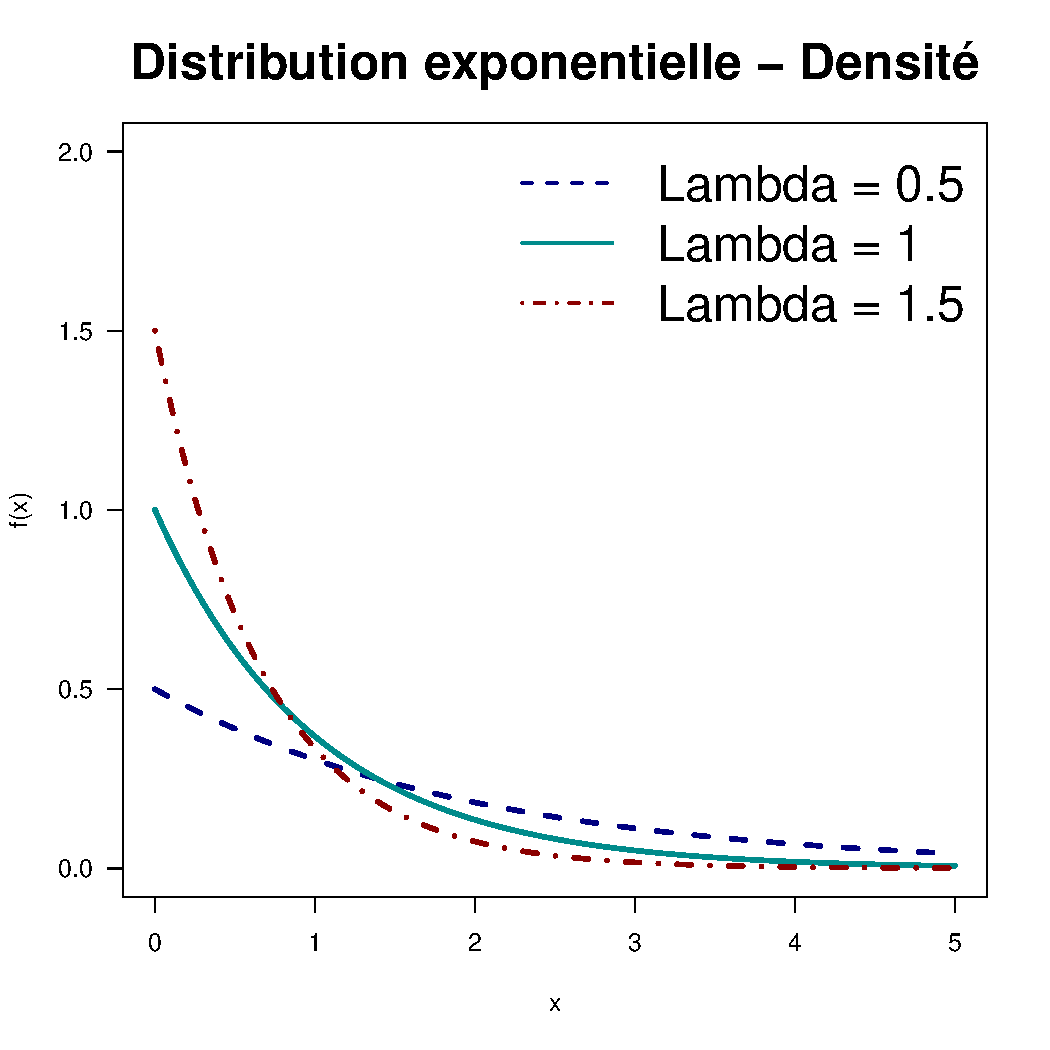
\includegraphics[scale=0.35]{Exp_pdf.pdf}
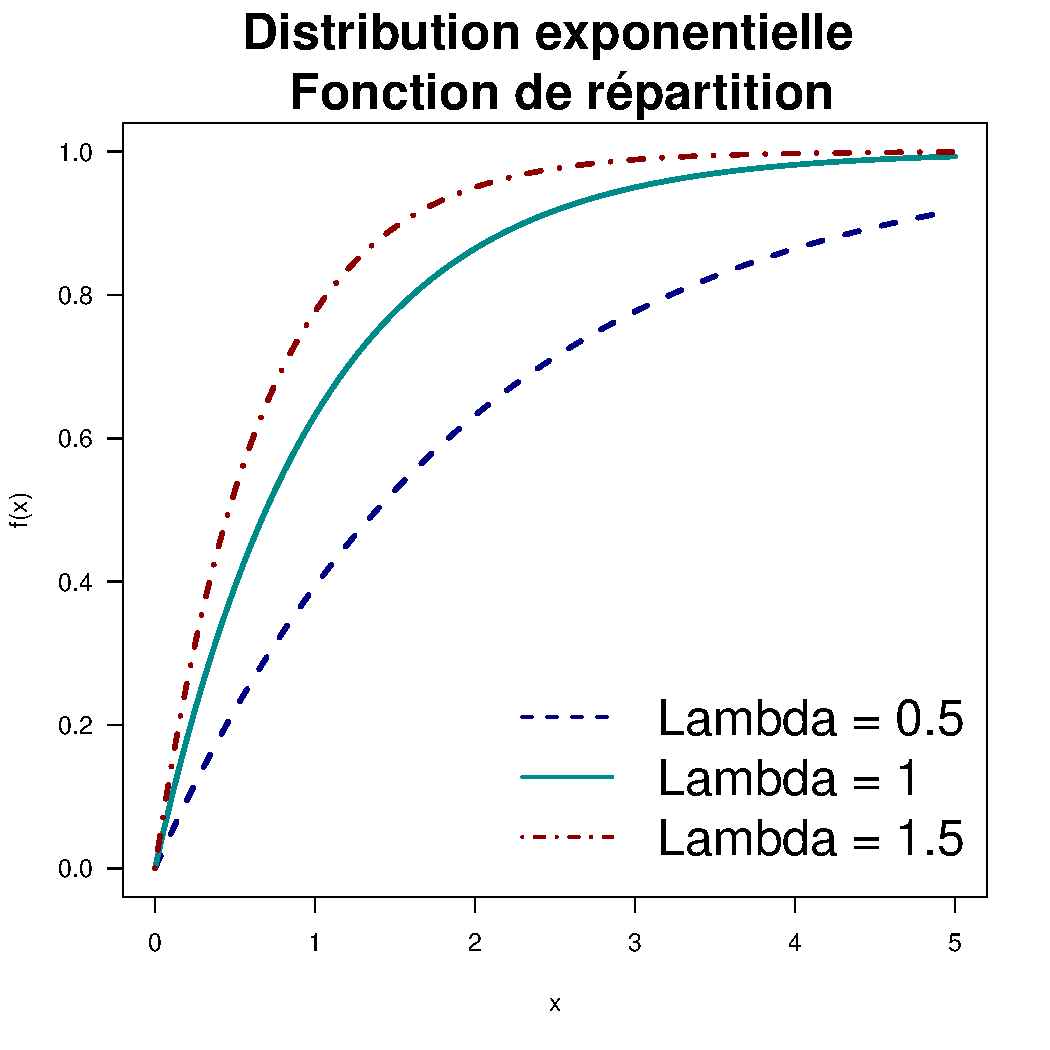
\includegraphics[scale=0.35]{Exp_cdf.pdf}


\end{frame}



\begin{frame}[t]{Exemple}

{\small
On suppose que le temps d'attente entre le passage de 2 bateaux sous un pont levis
suit une loi exponentielle de moyenne 3 heures. Quelle est la probabilité que plus
de 6 heures s'écoulent entre le passage de 2 bateaux?

\vspace{1in} Quelle est la probabilité
que 4 bateaux passent en 15 heures?
}
\end{frame}

\begin{frame}[t]{Loi exponentielle}
La loi exponentielle est \alerter{la seule loi continue
sans mémoire}:
\begin{align*}
P[X>x+s|X>s]&=\frac{P[X>x+s\text{\ et\ }X>s]}{P[X>s]}\\[8pt]
&=\frac{P[X>x+s]}{P[X>s]}
=\frac{1-F_X(x+s)}{1-F_X(s)}\\[8pt]
&=\frac{1-\{1-\exp(-\lambda\{x+s\})\}}
{1-\{1-\exp(-\lambda s)\}}=\frac{\exp(-\lambda\{x+s\})}{\exp(-\lambda s)}\\[8pt]
&=e^{-\lambda x-\lambda s -(-\lambda s)} =e^{-\lambda x} \\[8pt]
&=1-(1-e^{-\lambda x})\\[8pt]
&=P[X>x]
\end{align*}
\end{frame}

\begin{frame}[t]{Exemple}

{\small
La loi exponentielle est souvent utilisée pour modéliser la
durée de vie des ampoules électriques. On vous dit que la durée
de vie d'une certaine ampoule suit une loi exponentielle de moyenne 1000 heures.
On vous dit que cette ampoule fonctionne toujours après 500 heures. Quelle
est la probabilité qu'elle survivra au moins 1000 autres heures?
}
\end{frame}


\section{Loi Gamma}
 

\begin{frame}[t]{Loi Gamma}
Considérons $Y_1,\hdots,Y_n$ des variables aléatoires indépendantes et identiquement distribuées (i.i.d.), telles que $Y_i\sim \text{exp}(\lambda)$, $\forall i =1,\hdots,n$. Alors,
$$ X=\sum_{i=1}^nY_i  \sim \alerter{\mbox{Gamma}(n,\lambda)}.$$ 

\textbf{Fonction de densité:} Si $X \sim \mbox{Gamma}(n,\lambda)$, où $n>0$ et $\lambda > 0$, \\

$$f_X(x)=\left\{\begin{array}{ll}
\frac{\lambda}{\Gamma(n)}(\lambda x)^{(n-1)}e^{-\lambda x} & x > 0\\
0, & \text{sinon.}
\end{array}\right.$$
$\Gamma(r)$ est une fonction un peu complexe en général, mais pour un entier $n$ on a $\Gamma(n) = (n-1)!$
%Utilise la fonction Gamma

\vspace{0.2 in}
\textbf{Fonction de répartition:} N'a pas de forme explicite.
% doit être calculée à l'ordinateur.
%Donc, on ne calculera pas directement de prob pour cette loi.
\vspace{0.1 in}


\end{frame}

\begin{frame}{Loi Gamma}

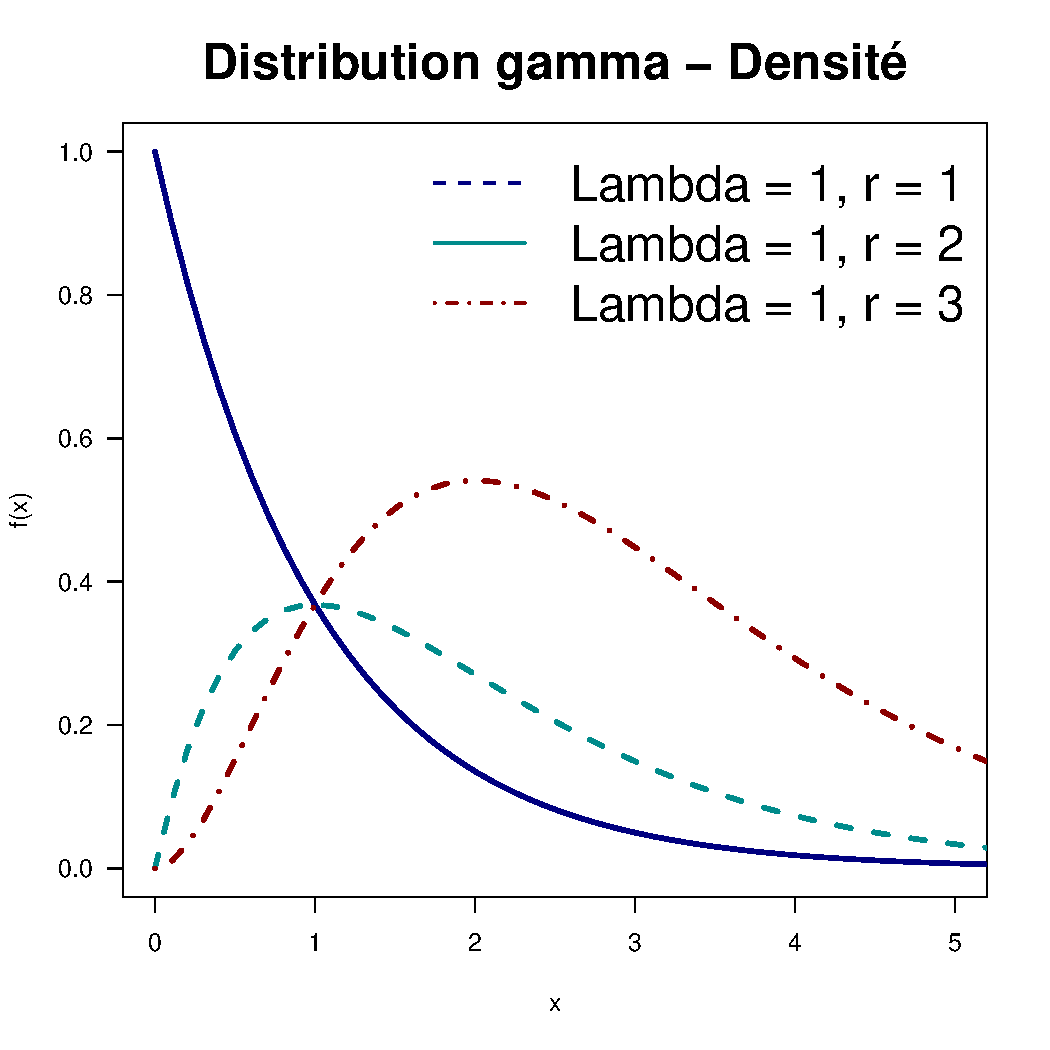
\includegraphics[scale=0.35]{Gamma_pdf.pdf}

*notez que le $r$ sur le graphique représente le $n$ dans la fonction de densité présentée plus haut
\end{frame}

\begin{frame}{Loi Gamma}

{\bf Espérance:} 
\vspace{-0.2 in}
$$E(X)=E(Y_1+\cdots+Y_n)=\sum_{i=1}^nE(Y_i)=
 \sum_{i=1}^n1/\lambda=n/\lambda$$



{\bf Variance:} 
\vspace{-0.5 in}
\begin{center}
\begin{align*}
V(X)&=V(Y_1+\cdots+Y_n)\\
&=\sum_{i=1}^nV(Y_i)+2\sum\sum_{i<j}Cov(Y_i,Y_j)\\
&=\sum_{i=1}^n1/\lambda^2+2\sum\sum_{i<j}0= \frac{n}{\lambda^2}
\end{align*}
\end{center}

 
\end{frame}




\begin{frame}{Lien avec les processus de Poisson}


Si les événements surviennent selon un processus de
Poisson de taux $\lambda$, alors on a que
\begin{itemize}
 \item le nombre d'événements dans tout intervalle
 de longueur $t$ est une v.a. suivant une loi de Poisson de
 moyenne $\lambda t$;
 \item le temps qui s'écoule entre deux événements (ou
 avant un premier événement)
 est une v.a. de loi exponentielle de paramètre $\lambda$ et donc de moyenne $1/\lambda$;
 \item  le temps qui s'écoule entre $n+1$ événements (ou
 avant un $n$-ème événement) est une v.a. qui suit une
 loi gamma$(n,\lambda)$.
\end{itemize}

\end{frame}

\begin{frame}[t]{En image}

    
\end{frame}

\begin{frame}[t]{Exemple}

{\small
Les temps que prend un hacker pour craquer des mots de passe peuvent
être vus comme des v.a. indépendantes de loi exponentielle de moyenne 15 minutes.
Quelles sont la distribution (loi), la moyenne et la variance du
temps qu'il prendra pour craquer les trois mots de passe qui protègent
un certain site? }
\end{frame}

\begin{frame}[t]{Exemple (suite)}

{\small
Si ce hacker a 20 minutes à sa disposition, quelle
est la probabilité qu'il craquera 2 mots de passes?
}

\end{frame}

\section{Loi de Weibull}

\begin{frame}[t]{Loi de Weibull}

{\small
La loi de  Weibull permet de modéliser une situation où la probabilité d'événement n'est pas constante dans le temps comme dans le cas de la loi exponentielle.  Par exemple, la probabilité de tomber en panne dans un instant donné ne reste pas constante dans le temps, mais augmente avec l'âge.\\

\vspace{0.1 in}
Le taux de cette augmentation peut être contrôlé par un des paramètres
de la loi (paramètre de forme).

\vspace{0.1in}
\smallskip

}
\end{frame}

\begin{frame}{Loi de Weibull}


Si $X$ suit une loi de Weibull($\delta,\beta,\gamma$) alors
$$f(x)=\left\{\begin{array}{ll}
\frac{\beta}{\delta}\left(\frac{x-\gamma}{\delta}\right)^{\beta-1}
\exp\left\{-\left(\frac{x-\gamma}{\delta}\right)^\beta\right\}, & x>\gamma\\
0, & \text{sinon}.\end{array}\right.$$


\vspace{0.2in}
On appelle $\beta$ ``paramètre de forme'' et $\delta$ ``paramètre
d'échelle''. \\

\vspace{0.5 in}
Si $\gamma=0$ et $\beta=1$, on retrouve la loi exponentielle de moyenne $\delta$!

\end{frame}

\begin{frame}{Fonction et répartition}
  
En posant $u=\{(s-\gamma)/\delta\}^\beta$ dans $\int_{-\infty}^xf(s)\;ds$, on
trouve
$$F(x)=\left\{\begin{array}{ll}
0, & x<\gamma\\
1-\exp\left\{-\left(\frac{x-\gamma}{\delta}\right)^\beta\right\}, & x\ge\gamma.
\end{array}\right.$$  

\vspace{0.4in} L'espérance et la variance de la loi de Weibull ont des formes un peu compliquées et ne sont pas à l'étude.
    
\end{frame}



\begin{frame}[t]{Exemple 1}

{\small
Les panneaux de verre installés sur un édifice ont des durées de vie
(en années) indépendantes et toutes de loi de Weibull$(20,2,0)$.
Ces panneaux sont vendus avec une garantie de 5 ans. Quelle est la probabilité
qu'un panneau ne dure pas jusqu'à la fin de sa garantie? } 
\end{frame}

\begin{frame}[t]{Exemple 1 (suite)}
S'il en co\^ute 1000\$ pour remplacer un panneau qui ne survit pas jusqu'à la fin de la garantie et que l'on vend 500 tels panneaux, quel est le co\^ut total espéré de la garantie?

\end{frame}

\begin{frame}[t]{Exemple 2}

{\small
On vous dit que la durée de vie de votre iPod (en années)
suit une loi de Weibull avec $\beta=3$, $\delta=4$ et
$\gamma=0$. \\
Quelle est la probabilité que votre iPod survive
au moins 3 autres années (i) s'il est neuf? (ii) s'il est
âgé de 2 ans?
}

\end{frame}

\begin{frame}[t]{Exemple 2 (suite)}

{\small
Quelle est la durée de vie médiane de tels iPod (c-à-d le
50ème percentile de la distribution, c-à-d le moment tel
que 50\% des iPod durent moins longtemps et 50\% des iPod durent
plus longtemps)?}

\end{frame}

\section{Loi normale}

\begin{frame}[t]{Loi normale}

\vspace{0.1in}
La loi normale est probablement la loi de probabilité la plus utilisée dans les
applications de la statistique. Quelques raisons de sa popularité:
\vspace{0.1 in}
\begin{itemize}
\item modélise bien la distribution de beaucoup de variables d'intérêt
\item approxime la loi de plusieurs variables aléatoires de nature complexe (théorème central limite)
\item mène à des résultats analytiques dans plusieurs problèmes d'inférence statistique
\end{itemize}
\end{frame}

\begin{frame}[t]{Loi normale}

La loi normale est définie par son espérance et sa variance.

\vspace{0.5 in}
Si $X$ suit une loi normale d'espérance
$\mu$ et de variance $\sigma^2$, dénoté
$X\sim \mathcal{N}(\mu,\sigma^2)$ alors

$$f(x)=\frac{1}{\sqrt{2\pi\sigma^2}}
e^{-\frac{1}{2}\left(\frac{x-\mu}{\sigma}\right)^2},\ \
-\infty<x<\infty.$$



\vspace{0.1 in}
Comme le nom des paramètres l'indique, on a alors 
$$E(X) = \mu$$ 
$$V(X) = \sigma^2$$

\bigskip
%\centerline{\includegraphics[height=6cm]{axesnorm.jpg}}
\end{frame}

\begin{frame}{Loi normale}
\begin{center}
    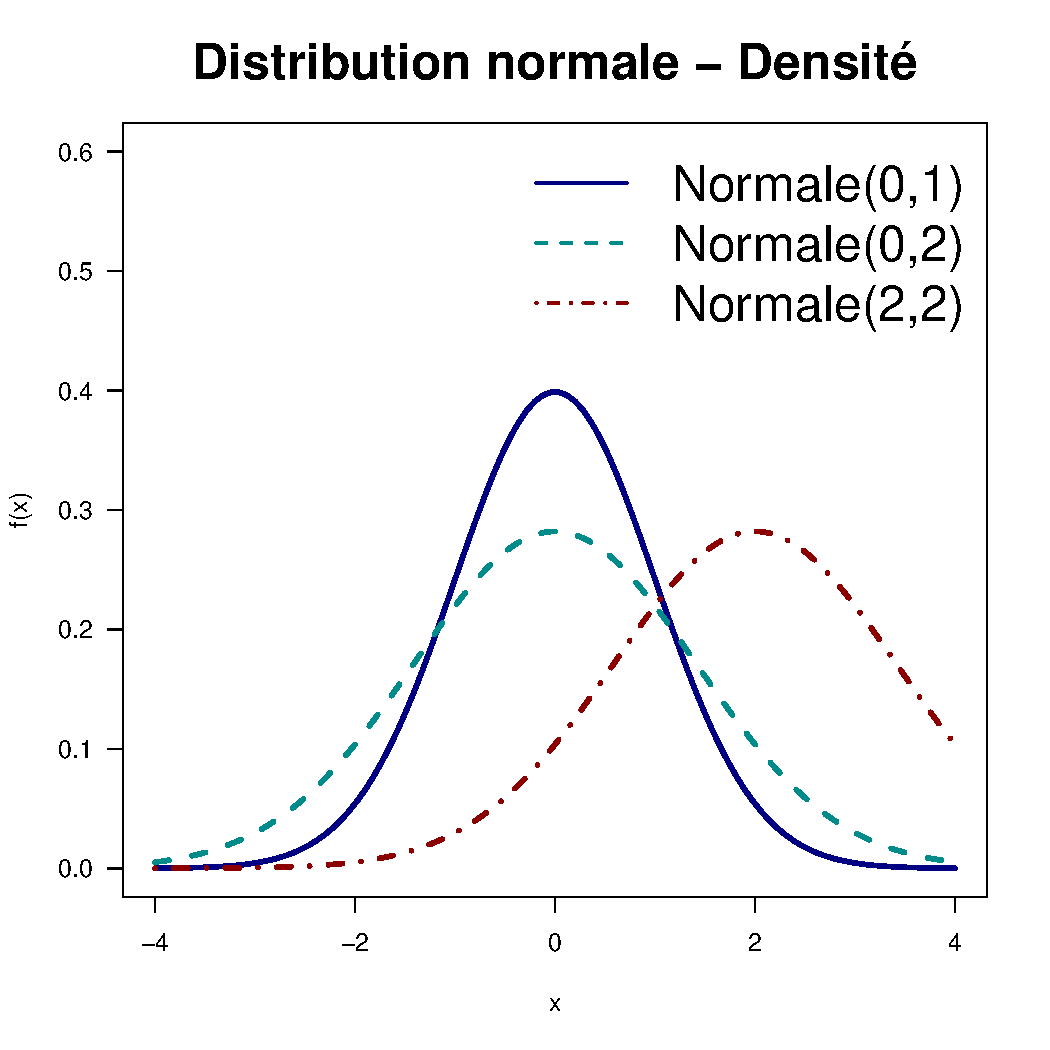
\includegraphics[scale = 0.3]{Normale_pdf.pdf}

\end{center}

\end{frame}

\begin{frame}[t]{Loi normale}

\vspace{0.3 in}
\begin{itemize}\itemsep12pt
\item $f(x)\ge0$ pour tout $x\in\mathbb{R}$
\item $\lim\limits_{x\to -\infty}f(x)=0$ et $\lim\limits_{x\to\infty}f(x)=0$
\item $f(\mu-x)=f(\mu+x)$ pour tout $x\in\mathbb{R}$, donc cette densité
est \alerter{symétrique autour de $\mu$}
\item $f(x)$ atteint son unique maximum en $x=\mu$
\item $f(x)$ a deux points d'inflexion, un en $\mu-\sigma$ et un en $\mu+\sigma$ (la deuxième dérivée est nulle)
\end{itemize}
\end{frame}



\begin{frame}[t]{Loi normale}

\vspace{0.2 in}
Rappel: Si $X\sim \mathcal{N}(\mu,\sigma^2)$ alors
$$f(x)=\frac{1}{\sqrt{2\pi\sigma^2}}
e^{-\frac{1}{2}\left(\frac{x-\mu}{\sigma}\right)^2},\ \
-\infty<x<\infty.$$

Donc, 
$$ F(x) = \int_{-\infty}^x \frac{1}{\sqrt{2\pi\sigma^2}}
e^{-\frac{1}{2}\left(\frac{t-\mu}{\sigma}\right)^2} dt$$

\vspace{0.2 in}
Il n'y a pas de solution analytique à cette intégrale. On doit obtenir ces valeurs à l'aide de logiciels, comme $\texttt{R}$ ou d'une table.

\end{frame}

\begin{frame}{Loi normale standard}

La loi $N(0,1)$ est appelée \alerter{loi normale standard} ou encore \alerter{loi normale centrée réduite}. Cette loi est très importante, et mérite donc une notation spéciale: 

\vspace{0.1 in}
Si $Z \sim N(0,1)$ alors on dénote

\begin{itemize}
\item  $\phi(z)$ la densité de $Z$\\[6pt]
$\phi(z)=(2\pi)^{-1/2}e^{-z/2}$ \\[12pt]
\item $\Phi(z)$ la fonction de répartition de $Z$\\[6pt]
$\Phi(z)$ n'a toujours pas de forme analytique, mais les livres de statistiques ont une table des valeurs de $\Phi(z)$. 
\end{itemize}


\end{frame}

\begin{frame}[t]{Loi normale standard}

\vspace{-1.2cm}
\hspace{-1.8cm}
\begin{center}
    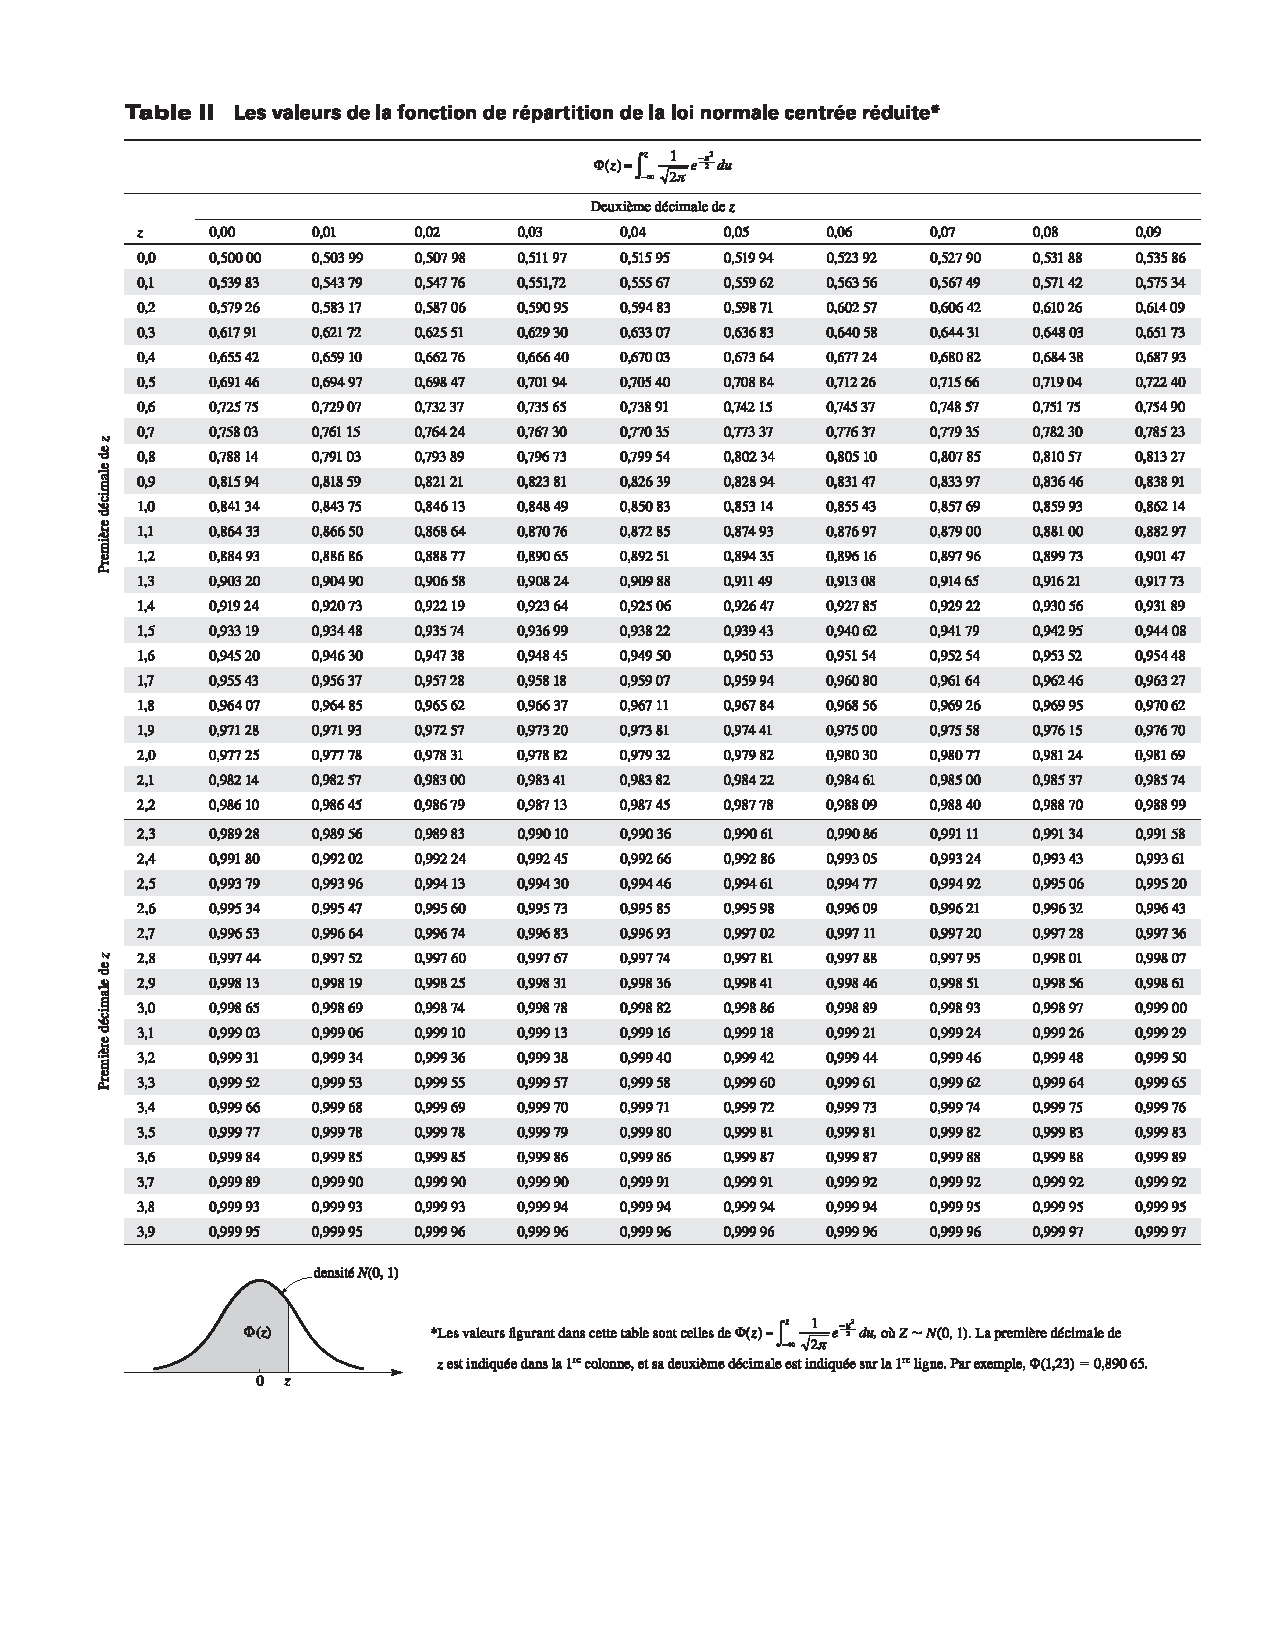
\includegraphics[height = 17cm, width = 12cm]{TableNormale.pdf}    
\end{center}



\end{frame}

\begin{frame}[t]{Loi normale standard}

On suppose que $X \sim N(0,1)$.

\vspace{0.1 in}
Quelle est la probabilité que $X$ soit plus petit que 1,15?

\vspace{1 in}
Quelle est la probabilité que $X$ soit plus grand que 1,15?



\end{frame}

\begin{frame}[t]{Loi normale standard}

Quelle est la probabilité que $X$ soit entre $0,4$ et $2,12$?
\vspace{1 in}

Quelle est la probabilité que $X$ soit plus petit que $-1,4$?



\end{frame}


\begin{frame}[t]{Loi normale standard}

Quelle est la probabilité que $X$ soit entre $-1,3$ et $1,98$?
\vspace{1 in}

Quelle est la probabilité que $|X|$ soit plus petit que 2?


\end{frame}

\begin{frame}[t]{Loi normale standard}

On peut aussi lire la table dans l'autre sens, i.e. trouver les valeurs de $x$ à partir des probabilités:
\vspace{0.1 in}

Quelle est la valeur $c$ telle que $P(X < c) = 78\%$?
\vspace{1 in}

Quelle est la valeur $c$ telle que $P(X > c) = 94,3\%$?

\end{frame}



\begin{frame}{Standardisation}

Si $X \sim N(\mu, \sigma^2)$, et qu'on veut calculer des probabilités pour $X$, on peut utiliser la table pour la loi normale standard grâce au processus de \alerter{standardisation}:

\begin{align*}
F_X(x)= P(X\le x)&=\int_{-\infty}^x \frac{1}{\sqrt{2\pi\sigma^2}}e^{-\frac{1}{2}(\frac{t-\mu}{\sigma})^2}dt\\[6pt]
&=\int_{-\infty}^{(x-\mu)/\sigma}\frac{1}{\sqrt{2\pi}}e^{-\frac{1}{2}z^2}\;dz\\[6pt]
&=\Phi\left(\frac{x-\mu}{\sigma}\right).
\end{align*}

\vspace{0.1in}
{\small Pour calculer la valeur de la fonction de répartition en $x$ pour une $N(\mu, \sigma^2)$, on peut simplement calculer la fonction de répartition de la loi normale standard en $\frac{x-\mu}{\sigma}$, par exemple à l'aide de la table.}

\end{frame}

\begin{frame}{Standardisation}
  
Un raisonnement similaire permet de montrer que si $$X\sim N(\mu,\sigma^2)$$
alors $$Z=\frac{(X-\mu)}{\sigma} \sim N(0,1).$$


\vspace{0.4 in}
 \alerter{$\Rightarrow$\ Seule une
table de la loi normale standard est requise!}  
   
\end{frame}


\begin{frame}[t]{Standardisation}
Supposons que $X\sim N(\mu,\sigma^2)$ et que l'on cherche
$P(a<X\le b)$.\\

\vspace{0.1 in}
 Alors si $Z=\frac{(X-\mu)}{\sigma}$, on a que $Z\sim N(0,1)$.
 
 Donc
\begin{align*}
P(a<X\le b)&=P\left(\frac{a-\mu}{\sigma}<\frac{X-\mu}{\sigma}\le
\frac{b-\mu}{\sigma}\right)\\[6pt]
&=P\left(\frac{a-\mu}{\sigma}<Z\le
\frac{b-\mu}{\sigma}\right)\\[6pt]
&=\Phi\left(\frac{b-\mu}{\sigma}\right)-\Phi\left(\frac{a-\mu}{\sigma}\right).
\end{align*}
\end{frame}

\begin{frame}[t]{Standardisation}


Les problèmes impliquant des calculs de probabilités pour la
loi normale se résolvent donc en deux étapes:\\
\begin{itemize}
\item[1-] standardiser la v.a. d'intérêt pour obtenir des probabilités impliquant la $N(0,1)$;\\
\item[2-] aller chercher les valeurs de $\Phi(\cdot)$ dans une table
\end{itemize}

\vspace{0.2in}

Comme la densité $N(0,1)$ est symétrique autour de 0, $$\Phi(-x)=1-\Phi(x) \mbox{ pour tout } x\in\mathbb{R}.$$ Les livres donnent donc généralement les valeurs de $\Phi(x)$ pour $x>0$.

%centerline{\includegraphics[height=4.5cm]{axesnorm01.jpg}}

\end{frame}

\begin{frame}[t]{Exemple 1}

{\small
La masse (en tonnes) des camions passant sur une viaduc peut être vue comme une v.a. normale de moyenne
50 et d'écart-type 10. \\

(i) Quelle est la probabilité qu'un camion pèse plus de 70 tonnes?
\vspace{1 in}

(ii) Quelle proportion des camions pèsent entre 40 et 60 tonnes? 
\vspace{1 in}
}
\end{frame}

\begin{frame}[t]{Exemple 1 (suite)}

{\small
(iii) Quelle est la masse, disons $m_1$, telle que 97.5\% des camions ont une masse inférieure à $m_1$? 
\vspace{1 in}

(iv) Quelle est la masse, disons $m_2$, telle que 97.5\% des camions ont une masse supérieure à $m_2$?
}
\end{frame}


\begin{frame}[t]{Loi normale}

\alerter{Une combinaison linéaire de variables aléatoires normales est aussi une variable aléatoire normale}, peu importe si les v.a. sont indépendantes ou pas.

\vspace{0.1 in}
On peut calculer sa moyenne et sa variance avec les formules vues précédemment pour les combinaisons linéaires de variables aléatoires. 


\vspace{0.1 in}
Par exemple, si $X_1,X_2,\ldots,X_n$ sont des v.a. \alerter{indépendantes} et que $X_i\sim N(\mu_i,\sigma^2_i)$ pour $i=1,\hdots,n$, alors 
$$ Y=X_1+X_2+\cdots+X_n \sim N\left( \sum_{i=1}^n \mu_i,\sum_{i=1}^n \sigma^2_i \right)$$
et
$$ W=a_1X_1+\cdots+a_nX_n \sim N\left( \sum_{i=1}^n a_i \mu_i,\sum_{i=1}^n a_i^2 \sigma^2_i \right) $$


\end{frame}

\begin{frame}[t]{Exemple 2}

{\small
Le portefeuille d'actions de votre firme est constitué à
20\% d'actions de ABC, 30\% d'actions de EFG et 50\% d'actions de
WXY. On vous dit que les rendements des trois titres sont des v.a.
normales indépendantes de variance 0.09 et de moyenne
0.12 pour ABC, 0.15 pour EFG et 0.15 pour WXY. Quelle est la probabilité
que le rendement global de ce portefeuille excède 0.17? \\
(Note: Le rendement global
du portefeuille est la combinaison linéraire des rendements
des actions individuelles dont les poids sont les proportions de chaque
action dans le portefeuille.)
}

\end{frame}

\begin{frame}[t]{Exemple 2 (suite)}


\end{frame}

\begin{frame}[t]{Un résultat très (très) utile}
\begin{thm}{}

Soit $X_1, X_2, ... X_n$ des variables aléatoires \alerter{indépendantes} de moyenne $\mu<\infty$, de variance $\sigma^2<\infty$, de loi de probabilité \alerter{quelconque}.
\vspace{0.5cm}

Alors si $n$ est assez grand (généralement $n \geq 30$),
\vspace{0.5cm}

$Y\;\;=\;\;X_1+\hdots+X_n\;\;\approx\;\; N(n\mu, n\sigma^2)$

\vspace{0.5cm}

$\overline X\;\;=\;\;\displaystyle\frac{X_1+\hdots+X_n}{n}\;\;\approx\;\; N\left(\mu, \frac{\sigma^2}{n}\right)$ 

\end{thm}
Nous appelons ce théorème, le \textit{théorème central limite} (TCL).
\end{frame}

\begin{frame}[t]
\begin{tabular}{p{5cm}|p{5cm}}

\alerter{1)} Vous pigez une boule dans une urne contenant 3 boules numérotées: 1, 2, 3.
& \alerter{2)} Vous remettez la boule dans l'urne et pigez une boule à nouveau.\\

\alerter{Vrai ou Faux?} & \alerter{Vrai ou Faux?}\\

{\it La valeur de la boule tirée a la distribution de probabilité suivante:}
& {\it La somme des deux numéros pigés a la distribution de probabilité suivante:}\\
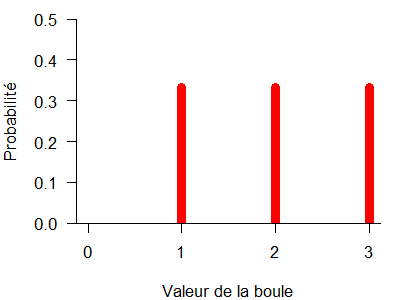
\includegraphics[width=4.5cm]{unif.png}
&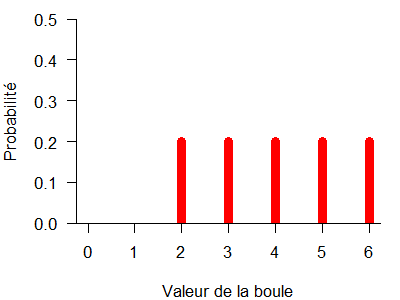
\includegraphics[width=4.5cm]{unif2.png}
\end{tabular}

\end{frame}

\begin{frame}[t]{Exemple 4}

{\small
Supposons que les demandes quotidiennes en électricité de 100 usines peuvent être
vues comme des v.a. indépendantes de moyenne 10 kWh et
d'écart-type 5 kWh. \\
Quelle est la probabilité approximative que la demande quotidienne totale en électricité de ces 100 usines excède la capacité de 1100 kWh du réseau qui les alimente ?}\\

\vspace{3.2cm}


\end{frame}

\begin{frame}[t]{Exemple 4 (solution)}

{\ \ \ }
\end{frame}


\section{Application : approximation de la loi binomiale par la loi normale}

\begin{frame}[t]{Idée générale}

Une v.a. binomiale peut être écrite comme une somme de v.a. indépendantes:
\vspace{1 in}

On peut donc approximer sa distribution par une loi normale:


\end{frame}

\begin{frame}[t]{Exemple}

Un étudiant fait une erreur de calcul dans 10\% de ses calculs. Si il doit répondre à un examen qui demande 100 calculs différents, quelle est la probabilité qu'il fasse plus de 5 erreurs de calcul?



\end{frame}

\begin{frame}[t]{Exemple (suite)}

Quelle est la probabilité que l'étudiant fasse exactement $5$ erreurs?\\



\end{frame}

\begin{frame}[t]{Correction pour la continuité}



Puisque la loi binomiale est discrète mais que la loi normale est continue, on doit faire une correction pour la continuité. 

\vspace{0.2 in}
Pour calculer $P(X=a)$ on calcule $P(a-0.5 \leq X \leq a+0.5)$:

\vspace{0.2 in}

De même pour les autres probabilités:\\

\begin{align*}
P(X \leq a) \approx \\
P(X < a) \approx \\
P(X \geq a) \approx \\
P(X > a) \approx  
\end{align*}

\end{frame}

\begin{frame}[t]{Exemple (suite) avec correction}

Un étudiant fait une erreur de calcul dans 10\% de ses calculs. Si il doit répondre à un examen qui demande 100 calculs différents, quelle est la probabilité qu'il fasse plus de 5 erreurs de calcul?  

\end{frame}


\begin{frame}{Bibliographie}
 	Ce document est rédigé avec Beamer ainsi qu'une classe .cls fourni par Jérôme Soucy. Les diapositives sont adaptées des diapositives créées par Anne-Sophie Charest 
 pour le cours STT-1000 ainsi que celles créées par Thierry Duchesne et Emmanuelle Reny-Nolin pour le cours STT-1900. Les graphiques proviennent de ces mêmes diapositives.
 	\printbibliography
 	\vfill
 	\footnotesize Pour signaler une erreur dans ce document, veuillez écrire à l'adresse :~\href{mailto:julien.miron@mat.ulaval.ca}{julien.miron@mat.ulaval.ca}.
 \end{frame}

\end{document}

